\documentclass{article}

\usepackage{geometry}
\usepackage{listings}
\usepackage{color}
\usepackage{titlesec}
\usepackage{biblatex}  
\addbibresource{ref.bib}

\setcounter{secnumdepth}{4}
\definecolor{dkgreen}{rgb}{0,0.6,0}
\definecolor{gray}{rgb}{0.5,0.5,0.5}
\definecolor{mauve}{rgb}{0.58,0,0.82}

\lstset{frame=tb,
  aboveskip=3mm,
  belowskip=3mm,
  showstringspaces=false,
  columns=flexible,
  basicstyle={\small\ttfamily},
  numbers=none,
  numberstyle=\tiny\color{gray},
  keywordstyle=\color{blue},
  commentstyle=\color{dkgreen},
  stringstyle=\color{mauve},
  breaklines=true,
  breakatwhitespace=true,
  tabsize=3
}



\usepackage{graphicx}
\usepackage{subfigure}
\usepackage{float}
\usepackage{tikz}
\usetikzlibrary{mindmap}

\setcounter{secnumdepth}{4}
\setcounter{tocdepth}{4}

\geometry{hmargin=2.5cm,vmargin=2.5cm}
\title{Projet : Blockchain appliquée au processus électoral}
\author{Yuxin XUE et Zhirui CAI}
\date{\today}

\begin{document}

\maketitle

\mbox{}
\hspace{15mm}

\begin{figure}[!b]
    \center
    \subfigure{
        \includegraphics[scale=0.6]{SUsciences.png}}
\end{figure}
\newpage

\tableofcontents
\newpage
\section{Introduction}
Ce projet vise à garantir le secret du vote lors de l'élection et à déterminer le vainqueur de manière équitable.\newline
Le déroulement du processus électoral a traditionnellement soulevé des questions de confiance et de transparence, et il est bien connu que le taux d'abstention aux élections est souvent relativement élevé.
Dans ce projet, nous souhaitons proposer une piste de réflexion sur les protocoles et sur les structures de données afin de mettre en œuvre efficacement le processus de détermination du vainqueur d'une élection, tout en garantissant l'intégrité, la sécurité et la transparence de l'élection.
\section{Description du code général}
\subsection{Code}
Nous utilisons make pour vérifier les dépendances et générer des exécutables ou des fichiers de bibliothèque.\newline
Le répertoire racine contient deux dossiers, `src` et `test`, `src` contenant le code source et `test` contenant les fichiers de test.
\begin{lstlisting}
Project:
│   makefile
├───scr
│       Makefile  │ utility.h
│       key.c       │       key.h		│       rsa.c        │       rsa.h
│       lcc.c        │       lcc.h		   │       sgn.c       │       sgn.h
│       lcp.c       │       lcp.h		  │      hash.c      │      hash.h
│       prime.c  │       prime.h	│      blo.c         │      blo.h
│       pro.c       │       pro.h	   	 │      blo_t.c      │      blo_t.h
│      sml.c        │      sml.h
└───test
    │  Makefile 
    │  key.c       lcp.c     lck.c       prime.c      pro.c       sgn.c       rsa.c
    │  blo.c		blo_t.c		sml.c		hash.c
    ├───blockchain
    │       block1.txt
    │		... ...
    └───temp
            blocks.txt		candidates.txt		declarations.txt		keys.txt
            Pending_block		Pending_votes.txt
            proof_of_work.csv		blocks_test.txt
\end{lstlisting}
\begin{itemize}
\item prime.c et prime.h contient des fonctions mathématiques qui génèrent des premiers dans un intervalle donné.
\item rsa.c et rsa.h contient les fonctions liées au protocole RSA, génère les valeurs des clés publiques et secrètes, encode et décode les messages.
\item key.c key.h contient la structure et les fonctions connexes des clés secrètes et publiques, initialise des clés secrètes et publiques, passe de la variable de la clé à sa représentation sous forme de chaîne de caractères et l'inverse
\item sgn.c et sgn.h contient la structure de la signature(Contient la clé secrète et le message codé) et les fonctions associées, initialise la signature, passe de la variable de la signature à sa représentation sous forme de chaîne de caractères et l'inverse.
\item pro.c et pro.h contient des structures protégées (c.-à-d. donnees protegees) et des fonctions connexes, initialise protected, passe des variables protected à leur représentation sous forme de chaîne et l'inverse. ils contient aussi Vérification de la validité de la signature (si le codage de la signature, une fois décodé, est le même que l'information stockée).
\item lck.c et lck.h contient la structure et les fonctions connexes pour cellKey (c'est-à-dire la liste chaînée de key), initialise CellKey, lit le fichier et génère la liste chaînée de key.
\item lcp.c et lcp.h contiennent la structure et les fonctions connexes de cellProtected (c'est-à-dire la liste chaînée de donnee Protégé), qui initialise cellProtected, lit le fichier et génère la liste chaînée de donnee Protégé. Le fichier contient également les fonctions utilisées pour générer les tests, telles que `generate\_random\_data`(qui est inclus dans pro.c) pour générer des données aléatoires.
\item blo.c et blo.h contiennent la structure et les fonctions associées pour `Block` (c'est-à-dire les blocs) et les fonctions pour générer les chaînes de hachage sha256 par chaîne, qui initialisent le Block, lisent et écrivent dans le fichier et génèrent les blocs.
\item blo\_t.c et blo\_t.h contiennent la structure du CellTree (c'est-à-dire l'arbre à blocs) et les fonctions associées qui initialisent l'arbre à blocs, lisent et écrivent les fichiers et génèrent l'arbre à blocs. Elles contiennent également des fonctions permettant d'ajouter des enfants à l'arbre parent et de mettre à jour la hauteur, de sélectionner l'enfant ayant la hauteur la plus élevée, le dernier nœud, de mélanger tous les CellProtected dans la plus longue chaîne
\item hash.c et hash.h contiennent la structure de la hashcell (i.e. case de hachage) hashtable (i.e. table de hachage) et les fonctions associées qui recherchent la position correspondante de la Clé et initialisent la table de hachage à partir de la CellKey. Finalement, le vainqueur est déterminé.
\item sml.c et sml.h contiennent des fonctions liées à la simulation du processus d'élection.
\item utility.h contien toutes les constantes utilisées dans le projet et peut être modifié en changeant le fichier pour changer les paramètres du projet et du test.
\item Dans le dossier de test, le nom du fichier de test est le même que le nom du fichier source.
\end{itemize}
Pour tous les free, nous utilisons valgrind pour nous assurer qu'il n'y a pas de fuites de mémoire.
\subsection{Description du processus d'élection}
Au début, pour les candidats et les électeurs, nous générons les clés secrètes et publiques pour chaque utilisateur. Ici, nous avons également besoin des volontaires pour compter les votes et nous les générons également.
\begin{enumerate}
\item Les électeurs envoient leurs votes. L'envoi se compose de la clé publique de l'électeur, du vote et de la signature, qui est chiffrée avec la clé privée de l'électeur. Une signature est considérée comme valide si et seulement si elle contient la même information que le vote après qu'il ait été décodé par une clé publique
\item Les informations relatives au vote sont cryptées par les clés secrètes  de l'électeur. Nous chiffrons le vote avec la clé secrète de l'électeur afin que n'importe qui puisse vérifier le vote avec la clé publique de l'électeur.
\item Les volontaires comptent les votes et les placent dans le bloc. Les blocs sont identifiés par le hachage et le hachage du bloc précédent.
\item Cryptage de blocs par preuve de travail. Un bloc n'est valable que si le travail s'avère conforme aux attentes, et nous préciserons plus tard comment cela fonctionne.
\item Ajout de blocs chiffrés à la blockchain. La blockchain est un arbre car le bloc peut avoir le même hash du bloc précédent que le bloc réel.
\item La chaîne la plus longue d'une blockchain est considérée comme la chaîne valide. En effet, les faux votes sont insérés de manière aléatoire dans un certain sous-arbre, mais il est difficile pour un faussaire de parvenir à forger directement plus de blocs que le nombre réel.
\item Vérifier la validité des votes (y compris la validité de la signature et la validité du bloc)
\item Détermination du gagnant par table de hachage
\end{enumerate}
\centerline{\includegraphics[scale=0.3]{processus.png}}
\section{Développement d’outils cryptographiques}
Dans cette section, nous allons développer quelques fonctions permettant de chiffrer des messages de manière asymétrique, à savoir : le système de cryptage à clé publique RSA.
\begin{itemize}
\item Une clé publique qui est transmise à l'expéditeur et qui lui permet de chiffrer son message.
\item Une clé secrète (ou privée), qui permet de décrypter le message à sa réception.
\end{itemize}
RSA (Rivest-Shamir-Adleman) est un système de cryptage à clé publique largement utilisé pour la transmission sécurisée de données.
Un utilisateur crée et publie une clé publique basée sur deux grands nombres premiers, ainsi qu'une valeur auxiliaire. 
Les nombres premiers sont tenus secrets. Les messages peuvent être cryptés par n'importe qui, via la clé publique, mais ne peuvent être décodés que par quelqu'un qui connaît les nombres premiers.
\subsection{Résolution du problème de primarité}
Les clés publiques et privées nécessitent des nombres premiers. Nous allons donc commencer par générer des nombres premiers. 
La méthode que nous utilisons est très simple, nous générons d'abord un nombre aléatoire, puis si le nombre généré n'est pas un nombre premier, nous générons un autre nombre aléatoire... jusqu'à ce que le nombre soit un nombre premier.
Il est donc particulièrement important de choisir la fonction qui détermine si c'est un nombre premier. Deux méthodes ont été développées. Commençons par la méthode classique.
\subsubsection{Implémentions par une méthode naıve}
par le calcul de $a^m$ valeurs (qui peuvent être très grandes), une approche naïve serait de
\begin{enumerate}
\item multiplier la valeur actuelle par a.
\item appliquer modulo n au résultat avant de passer à l'itération suivante
\end{enumerate}
Répétez ces opérations m fois.
\begin{lstlisting}[language={C}]
int  is_prime_naive(long p);
long modpow_naive(long a, long m, long n);
\end{lstlisting}
\begin{itemize}
\item int is\_prime\_naive(long p) teste si p est premier. Sa complexité est en O(p/2).
\item long modpow\_naive(long a, long m, long n) qui retourne la valeur $a^b$ mod n en la multipliant par a à chaque itération
\end{itemize}
Pour tester la vitesse de cette fonction, nous exécutons is\_prime\_naive pour chaque entier afin de trouver le plus grand nombre premier qui peut être exécuté en deux millièmes de seconde.
\addcontentsline{toc}{paragraph}{Q1.2}
\paragraph*{Q1.2}
Après 6 tentatives, nous sommes finalement parvenus à un nombre maximal de nombres premiers pouvant être testés en 2 millisecondes d'environ 32329 qui est beaucoup plus petit que la limite supérieure de la fourchette de nombres souhaitée($2^16$).\newline
\begin{table}[H]
\centering
\begin{tabular}{|l|l|l|l|l|l|l|}
\hline
fois    & 1     & 2     & 3     & 4     & 5     & 6     \\ \hline
premier & 32329 & 31261 & 30639 & 31515 & 30973 & 36153 \\ \hline
\end{tabular}
\caption{le plus grand nombre premier a tester en moins de 2 millièmes}
\end{table}
\newline Nous souhaitons donc améliorer cet algorithme. Au lieu de multiplier par a à chaque itération, il est en fait possible d'élever au carré (directement avec modulo), ce qui donne un algorithme d'une complexité logarithmique (c'est-à-dire O(log2(m)).\newline
ab mod n est égal à .
\begin{enumerate}
\item retourne 1 lorsque m = 0 (cas de base).
\item b ∗ b mod n avec b = am/2 mod n, lorsque m est pair.
\item a ∗ b ∗ b mod n avec b = a⌊m/2⌋ mod n, lorsque m est impair.
\end{enumerate}
Nous allons comparer la vitesse de ces deux méthodes à l'aide de calculs pratiques.
\begin{lstlisting}[language={C}]
long modpow(long a, long m, long n);
\end{lstlisting}
\begin{itemize}
\item int modpow(long a, long m, long n) retourne la valeur $a^b$ mod n par des élévations au carré
\end{itemize}
\addcontentsline{toc}{paragraph}{Q1.3}
\paragraph*{Q1.3}
Pour modpow\_naive qui retourne la valeur $a^b$ mod n, on fait m tours de boucle. Comme les opérations à l'intérieur de la boucle sont à nombre constant et sont en O(1),alors on peut conclure que la complexité est O(m).
\addcontentsline{toc}{paragraph}{Q1.5}
\paragraph*{Q1.5}
\centerline{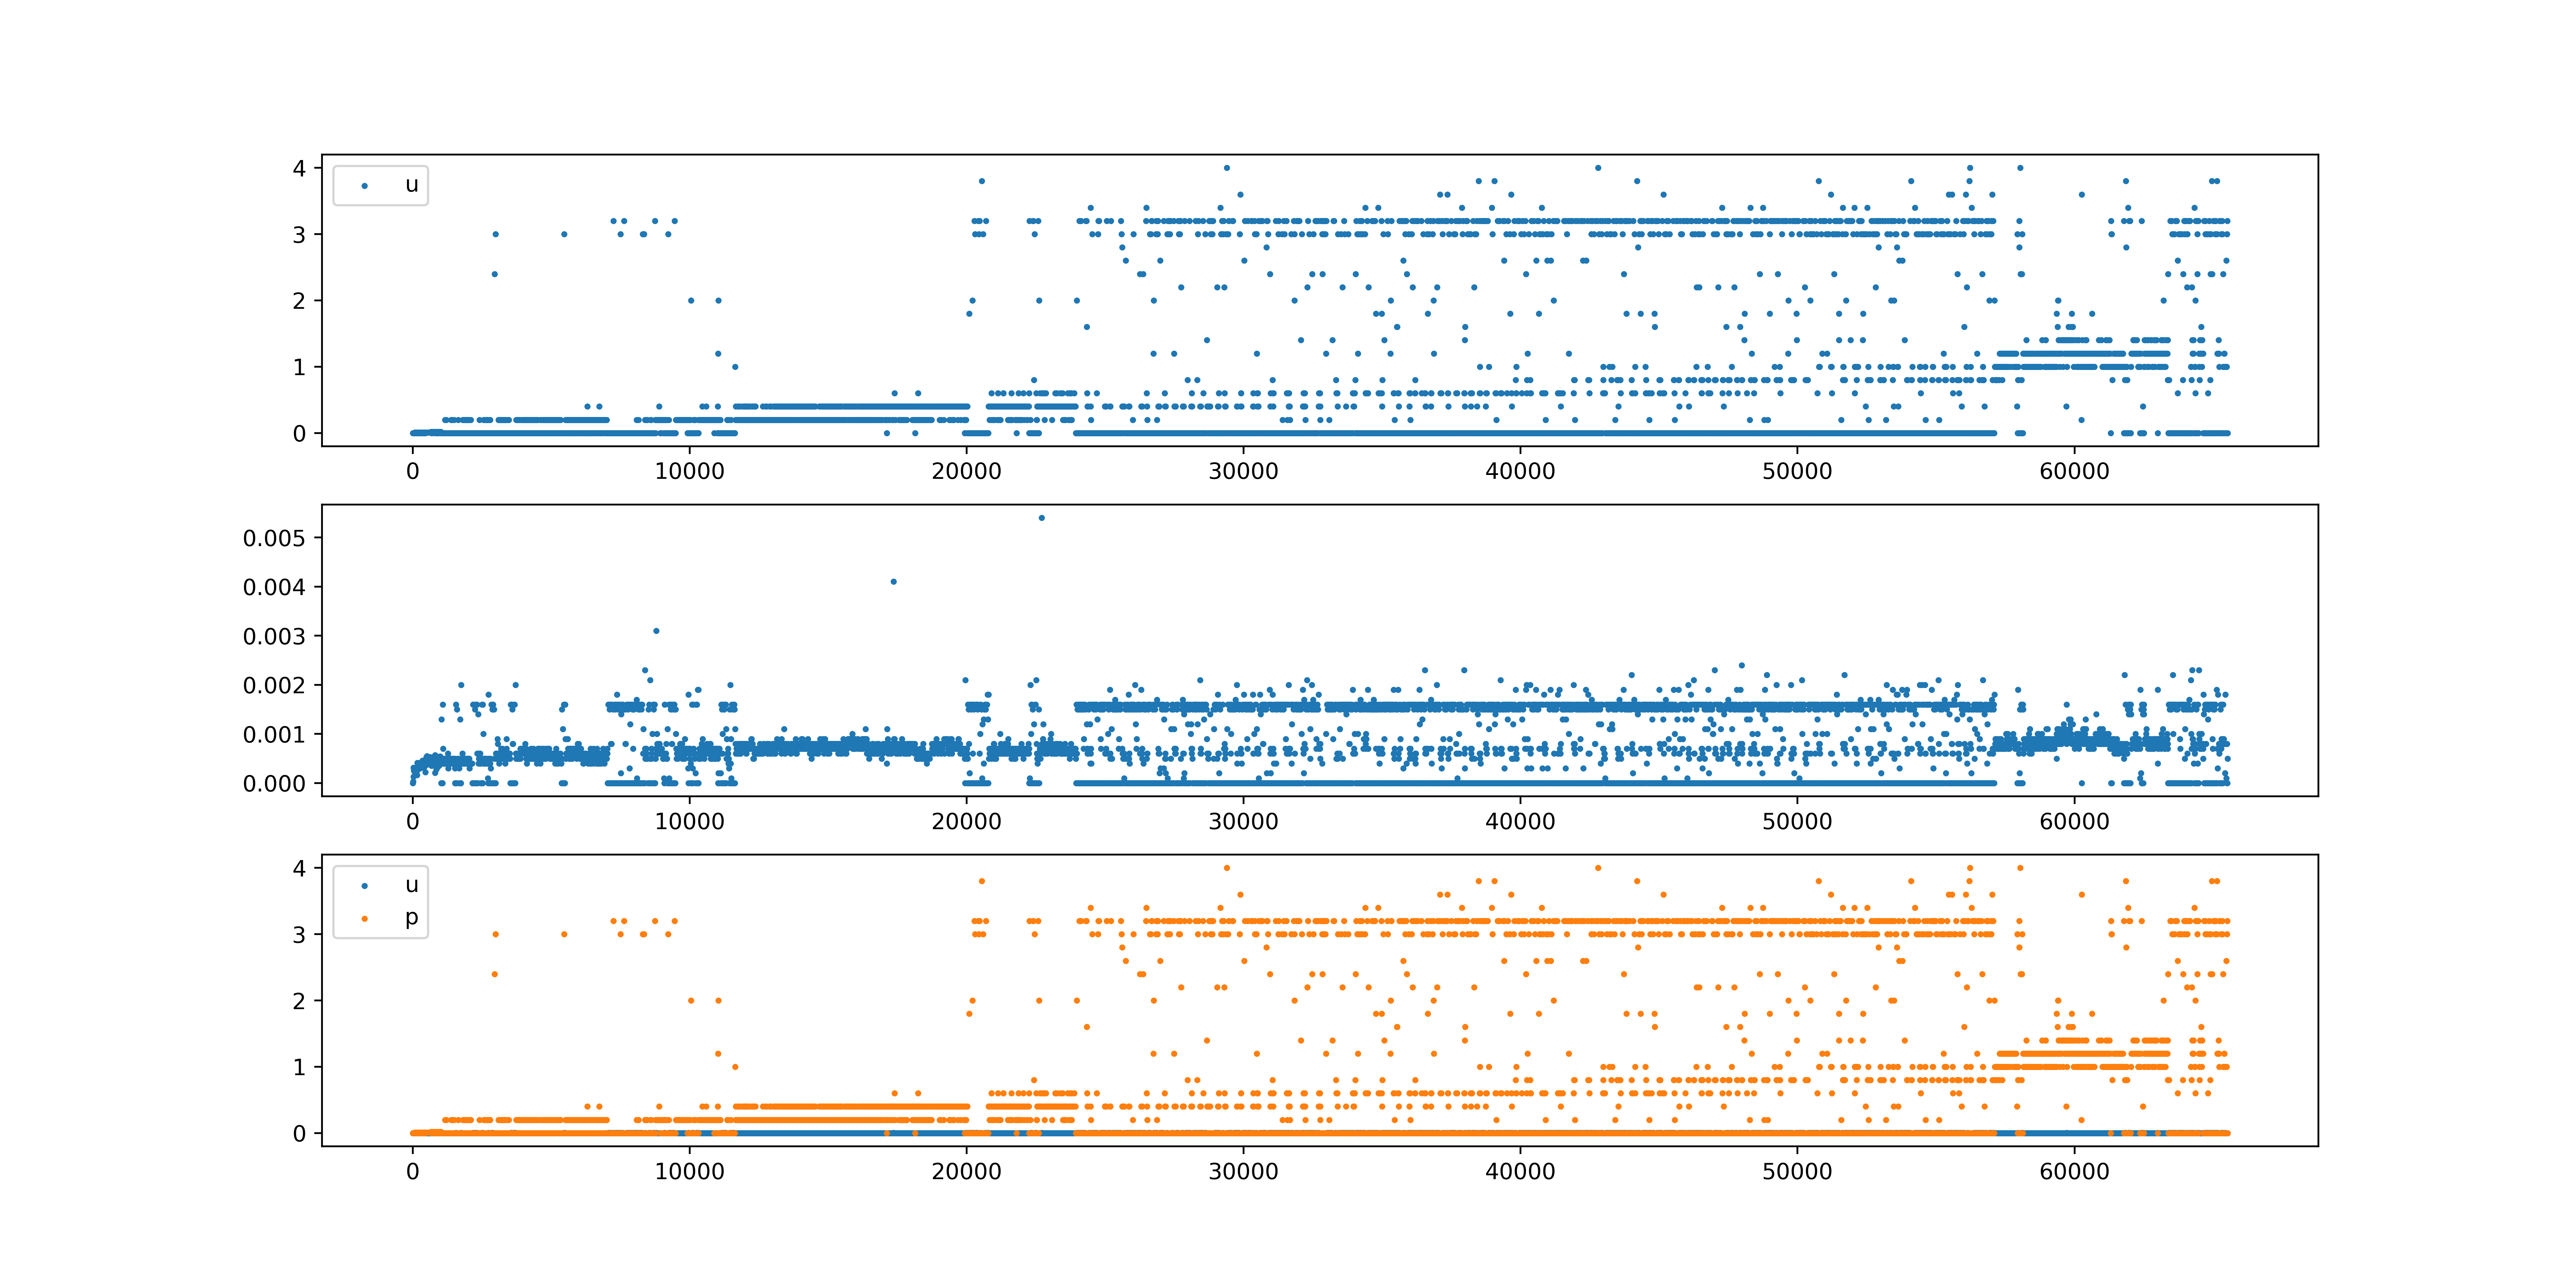
\includegraphics[scale=0.3]{q1_5.png}}
\centerline{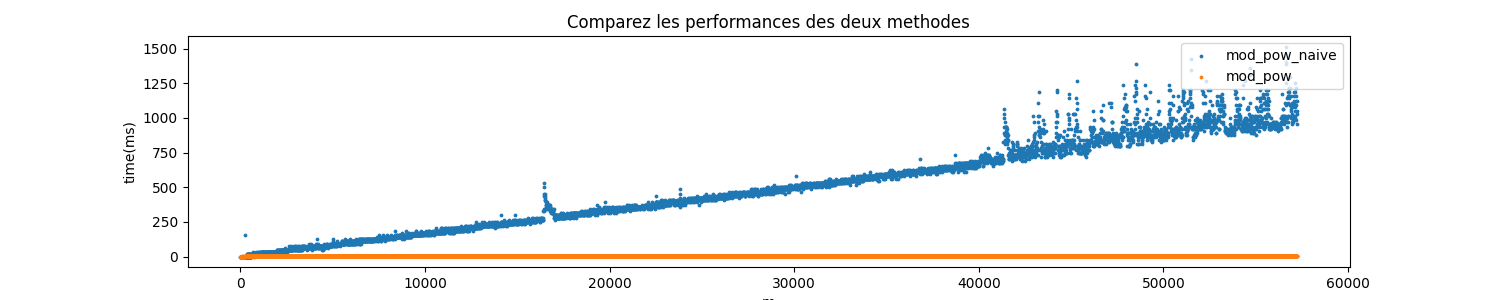
\includegraphics[scale=0.3]{q1_5_2.png}}
\newline
Sur la base de ces deux courbes, nous pouvons voir que modpow est beaucoup plus rapide que modpow\_naive, dont la vitesse varie moins. Nous pouvons conclure que modpow est plus efficace que modpow\_naive.
\subsubsection{Implémentions du test de Miller-Rabin}
Le test de primauté de Miller-Rabin utilise un algorithme de randomisation pour déterminer si un nombre est premier ou non.
Le test de Miller-Rabin s'appuie sur le fait que dans un corps, ce qui est le cas de ℤ/pℤ si p est premier, l'équation $X^2 = 1$ n'a pour solutions que 1 et –1. 
Soit p un nombre impair quelconque. Soit s et d deux entiers tels que $p = 2^b\cdot d + 1$. Supposons que a soit un entier strictement inférieur à p. \newline
Si nous pouvons trouver un tel a satisfaisant les deux équations ci-dessous:
\begin{itemize}
\item $a^d mod n=1$
\item $a^{2^r\cdot d} mod n =1$
\end{itemize}

alors n n'est pas un nombre premier. On dit que a est la témoin de Miller de p.\newline
\begin{lstlisting}[language={C}]
int  witness(long a, long b, long d, long p);
int  is_prime_miller(long p, int k);
long random_prime_number(int low_size, int up_size, int k);
\end{lstlisting}
\begin{itemize}
\item int witness(long a, long b, long d, long p) utilise la fonction modpow pour teste si a est un témoin de Miller pour
p, pour un entier a donné.
\item long rand\_long(long low, long up) retourne un entier long généré aléatoirement entre low et up inclus.
\item int is\_prime\_miller(long p, int k) utilise witness et rand\_long pour réaliser le test de Miller-Rabin en générant k valeurs de a au hasard, et en testant si chaque valeur de a est un témoin de Miller pour p. La fonction retourne 0 dès qu’un témoin de Miller est trouvé (p n’est pas premier), et retourne 1 si aucun témoin de Miller n’a été trouvé (p est très probablement premier).
\item long random\_prime\_number(int low\_size, int up\_size, int k) retourne un nombre premier de taille comprise entre low\_size et up\_size en utilisant rand\_long et is\_prime\_miller  .
En raison du caractère aléatoire utilisé dans cette méthode, nous devons connaître son erreur
\end{itemize}

\addcontentsline{toc}{paragraph}{Q1.7}
\paragraph*{Q1.7}
En utilisant le fait que, pour tout entier p non premier quelconque, au moins 3/4 des valeurs entre 2 et p-1 sont des témoins de Miller pour p. \newline
Nous pouvons conclure que la probabilité que l'un des nombres choisis au hasard ne soit pas un témoin de Miller est de 1/4. Étant donné que dans l'algorithme nous testons k fois de suite, la probabilité que tous les nombres testés ne soient pas des témoins de Miller est de $(\frac{1}{4})^k$.\newline
une borne supérieure sur la probabilité d’erreur de l’algorithme est $(\frac{1}{4})^k$.
L'erreur décroît de manière exponentielle, et est déjà faible lorsque k est supérieur à 20.

\subsection{Implémentions du protocole RSA}
\subsubsection{Génération d'une clé publique et d'une clé secrète}
Pour pouvoir envoyer des données confidentielles à l'aide du protocole RSA, il est d'abord nécessaire de générer deux clés : une clé publique pour chiffrer le message et une clé secrete pour le déchiffrer.Afin de sécuriser l'échange, une couple (clé secrète, clé publique) doit être générée de telle sorte qu'il soit impossible, de récupérer la clé secrète à partir de la clé publique. Le fonctionnement du protocole RSA est basé sur la difficulté de factoriser de grands nombres entiers. Plus précisément, afin de générer une couple(clé secrète, clé publique), le protocole RSA requiert deux (grands) nombres premiers distincts p et q (générés au hasard) et effectue les opérations suivantes:
\begin{enumerate}
    \item Calculer n = p × q et t = (p-1) × (q-1).
    \item Générer aléatoirement des entiers s inférieur à t jusqu'à en trouver un tel que PGCD(s, t) = 1.
    \item Déterminer u tel que s × u mod t = 1.
\end{enumerate}
Le couple pkey = (s, n) constitue alors la clé publique, tandis que le couple skey = (u, n) forme la clé secrète.\newline
\begin{lstlisting}[language={C}]
void  generate_key_values(long p, long q, long *n, long *s, long *u);
long  extended_gcd(long s, long t, long *u, long *v);
\end{lstlisting}
\begin{itemize}
\item La fonction generate\_key\_values(long p, long q, long* n, long *s,long *u)utilise rang\_long(dans libp.c) et extended\_gcd pour génère la clé publique pkey = (s, n) et la clé secrète skey = (u, n), à partir des nombres premiers p et q, en suivant le protocole RSA.
\end{itemize}

\subsubsection{Chiffrement et déchiffrement de messages}
Dans cette section, nous nous concentrons sur la manière de déchiffrer des messages à l'aide d'une clé secrète sKey=(u,n)  et de les chiffrer à l'aide d'une clé publique pKey=(s,n).
\begin{itemize}
\item Chiffrement : on chiffre le message m en calculant c = $m^s$ mod n (c est la représentation
chiffrée de m).
\item Déchiffrement : on déchiffre c pour retrouver m en calculant m = $c^u$ mod n.
\end{itemize}
\begin{lstlisting}[language={C}]
long *encrypt(char *chaine, long s, long n);
char *decrypt(long *crypted, int size, long u, long n);
void  print_long_vector(long *result, int size);
\end{lstlisting}
\begin{itemize}
\item La fonction encrypy chiffre la chaîne de caractères avec la clé publique.
\item La fonction decrypy déchiffre la chaîne de caractères avec la clé secrète.
\item La fonction print\_long\_vector est de tester la validité de la fonction ci-dessus
\end{itemize}

Pour le tester, nous créons une paire de clés secrètes et publiques, nous codons et décodons un message donné (par exemple "hello") et nous comparons les messages codés et décodés pour voir s'ils correspondent au message original.
\section{Déclarations sécurisée}
Dans cette partie,on s'intéresse au problème de vote.On va supposer que l'ensemble de candidats est déjà connu, et que les citoyens ont juste à soumettre des déclarations de vote.\newline
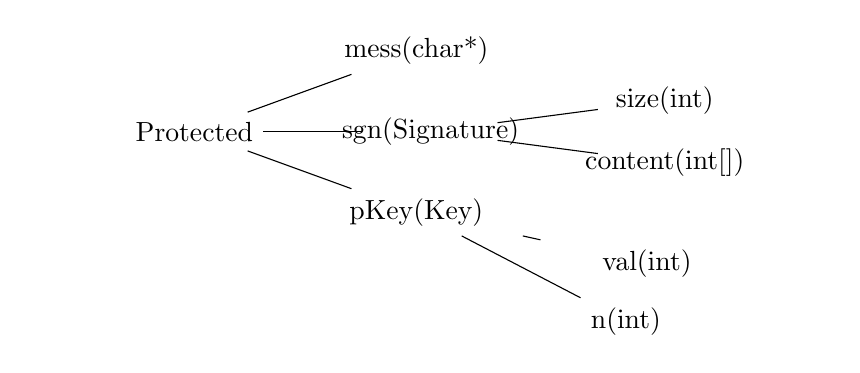
\begin{tikzpicture}[grow cyclic, text width=4cm, align=flush center,
	level 1/.style={level distance=3cm,sibling angle=20},
	level 2/.style={level distance=3cm,sibling angle=15}]
\node{Protected}
child { node {pKey(Key)}
	child { node {n(int)}}
	child { node {val(int)}}
}
child { node {sgn(Signature)}
	child { node {content(int[])}}
	child { node {size(int)}}
}
child { node {mess(char*)}
};
\end{tikzpicture}
\subsection{Manipulations de structures sécurisées}
Dans notre modèle, chaque citoyen possède une carte électorale, qui est définie par un couple de clés :
\begin{itemize}
    \item Une clé secrète (ou privée) qu’il utilise pour signer sa déclaration de vote. Cette clé ne doit être connue que par lui.
    \item Une clé publique permettant aux autres citoyens d’attester de l’authenticité de sa déclaration (vérification de la signature). Cette clé est aussi utilisée pour l’identifier dans une déclaration de vote, non seulement quand il vote, mais aussi quand quelqu’un souhaite voter en sa faveur.
\end{itemize}
\subsubsection{Manipulation de clés}
Dans le protocole RSA, la clé public et la clé secrète d’un individu sont des couples d’entiers, notés respectivement pKey = (s, n) et sKey = (u, n). On écrit des fonctions pour initialiser des clés et passer d'un clé à sa représentation sous forme de chaîne de caractères et inversement. 
\begin{lstlisting}[language={C}]
typedef struct _Key {
    long val;
    long n;
} Key;

void  init_key(Key *key, long val, long n);
void  init_pair_keys(Key *pKey, Key *sKey, int low_size, int up_size);
char *key_to_str(Key *key);
Key  *str_to_key(char *str);
\end{lstlisting}
\begin{itemize}
    \item La fonction init\_key attribuer des valeurs à la clé qui est déjà allouée.
    \item La fonction init\_pair\_keys utilise random\_prime\_number (dans libp.c) pour générer deux premiers aléatoires, puis utiliser generate\_key\_values (dans rsa.c) pour créer les valeurs des clés secrète et publique, et enfin utilise init\_key pour créer les clés secrète et publique.
    \item La fonction key\_to\_str  passe d'un clé à sa représentation sous forme de chaîne de caractères.
    \item La fonction str\_to\_key passe d'un chaîne de caractères à clé.
\end{itemize}
\subsubsection{Signature}
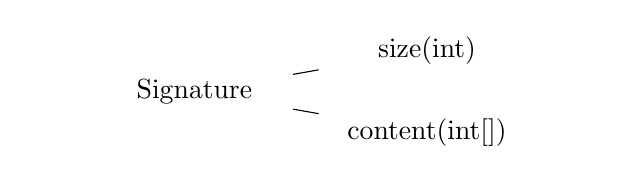
\begin{tikzpicture}[grow cyclic, text width=4cm, align=flush center,
	level 1/.style={level distance=3cm,sibling angle=20},
	level 2/.style={level distance=3cm,sibling angle=15}]
\node{Signature}
	child { node {content(int[])}}
	child { node {size(int)}
    };
\end{tikzpicture}\newline
Dans cette section, chaque électeur doit produire une déclaration de vote signée pour garantir son authenticité. Cette signature consiste en un tableau de long, gérée par l'émetteur de la déclaration au moyen de sa clé secrète, qui peut être vérifiée par d'autres personnes au moyen de la clé publique de l'émetteur.Le protocole de déclaration de vote:\newline
Avant de publier la déclaration, on génère la signature associée à sa déclaration de vote. Cette signature prendra la forme d’un tableau de long obtenu par chiffrement du message mess avec la clé secrète de l’électeur.\newline
L’électeur peut ensuite publier une déclaration sécurisée, composée de sa déclaration mess, de la signature associée, et de sa cl´e publique.Ceux qui souhaitent vérifier l'authenticité de la déclaration peuvent déchiffrement la signature en utilisant la clé publique de l'électeur.\newline
\begin{lstlisting}[language={C}]
typedef struct signature {
    int   size;
    long *content;
} Signature;

Signature *init_signature(long *content, int size);
Signature *sign(char *mess, Key *sKey);
char      *signature_to_str(Signature *sgn);
Signature *str_to_signature(char *str);
void       free_signature(Signature *sgn);
\end{lstlisting}
Les fonctions ont presque la même structure que la clé.
\begin{itemize}
    \item free\_signature libere la memoire de Signature.
\end{itemize}
\subsubsection{Déclarations signées}
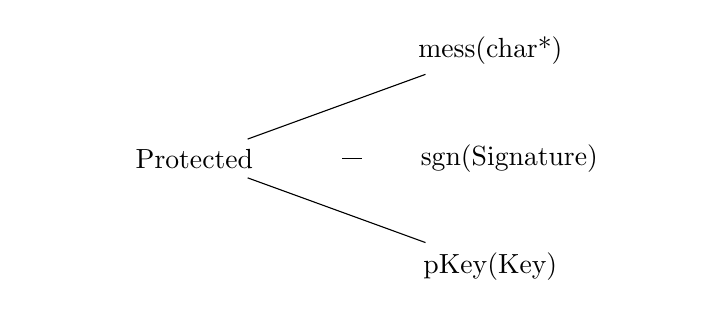
\begin{tikzpicture}[grow cyclic, text width=4cm, align=flush center,
	level 1/.style={level distance=4cm,sibling angle=20},
	level 2/.style={level distance=4cm,sibling angle=15}]
\node{Protected}
child { node {pKey(Key)}
}
child { node {sgn(Signature)}
}
child { node {mess(char*)}
};
\end{tikzpicture}
\newline On crée des déclarations signées en utilisant la structure Protected qui contient la clé publique de l'électeur, sa déclaration de vote, et la signature associée.
\begin{lstlisting}[language={C}]
typedef struct _Protected {
    Key       *pKey;
    Signature *sgn;
    char      *mess;
} Protected;

Protected *init_protected(Key *pKey, char *mess, Signature *sgn);
int        verify(Protected *pr);
char      *protected_to_str(Protected *sgn);
Protected *str_to_protected(char *str);
void       free_protected(Protected *pr);
\end{lstlisting}
les fonctions ont aussi presque la même structure que la clé.
\begin{itemize}
    \item free\_signature libere la memoire de Protection.
    \item La fonction verify vérifie que la contenue dans signature correspond bien au message contenus apres decoder.
\end{itemize}
Pour tester la validité de ces fonctions, nous générons d'abord les clés secrètes et publiques, puis les signatures et les déclarations, et nous vérifions que les informations stockées dans les déclarations correspondent aux informations originales lorsqu'elles sont décodées.

\subsection{Création de données pour le processus de vote}
Nous allons simuler une séance de vote.Chaque citoyen aura une carte électorale unique contenant sa clé secrète et une clé publique.  Le citoyen votera avec sa clé secrète pour garantir son anonymat. Le système de vote recueillera ces déclarations signées et utilisera toutes les clés publiques recueillies pour vérifier leur authenticité.
\begin{enumerate}
\item Générer nv paires de clés différentes (publique, secrète), représentant nv citoyens.
\item Créez un fichier key.txt contenant toutes ces paires de clés (une paire par ligne).
\item candidats sont élus en public afin de garantir leur sécurité.
\item Créez un fichier candidats.txt contenant les clés publiques de tous les candidats (une clé publique par ligne).
\item générer un bulletin de vote signé pour chaque citoyen (candidat sélectionné au hasard).
\item Créez un fichier declarations.txt contenant toutes les déclarations de signature (une déclaration par ligne).
\end{enumerate}
\begin{lstlisting}[language={C}]
void generate_random_data(int nbCitoyen, int nbCandidate);
\end{lstlisting}
\begin{itemize}
    \item La fonction generate\_random\_data créer des données aleatoir
\end{itemize}
\section{Base de déclarations centralisée}
Dans cette section, nous allons créer un système de vote centralisé qui collectera toutes les déclarations de vote et annoncera ensuite le gagnant aux citoyens.Toutes les déclarations de vote seront incluses dans un fichier appelé declarations.txt, qui sera ensuite stocké dans un tableau lié. Afin de pouvoir vérifier l'intégrité des données et compter les votes, le système doit également récupérer toutes les clés publiques des citoyens et des candidats, qui sont stockées dans des fichiers appelés respectivement keys.txt et candidents.txt.\newline
\subsection{Lecture et stockage des données dans des listes chaînées}
Dans cette section, nous allons lire les fichiers keys.txt et candidates.txt afin de récupérer les clés. Nous allons ensuite lire le fichier declarations.txt pour récupérer les déclarations signées.\newline
\subsubsection{Liste chaînées de clés}
Nous allons créer des fonctions pour lire les fichiers contenant des clés et les stocker sous forme de listes chaînées.\newline
Enfin, nous testons toutes les déclarations contenues dans ce fichier, dans le but de supprimer toutes les déclarations invalides (c'est-à-dire que le codage dans la signature est décodé différemment de l'information correcte)\newline
\begin{lstlisting}[language={C}]
typedef struct cellKey {
    Key            *data;
    struct cellKey *next;
} CellKey;
CellKey *create_cell_key(Key *key);
CellKey *read_public_keys(char *fichier);
void     print_list_keys(CellKey *LCK);
void     delete_cell_key(CellKey *c);
void     delete_list_key(CellKey *LCK);
void add_head(CellKey **LCK, Key *key);
\end{lstlisting}
\begin{itemize}
    \item La fonction create\_cell\_key Alloue et initialise une cellule de liste chaînée.
    \item La fonction read\_public\_keys Prend en entrée le fichier keys.txt ou le fichier candidates.txt, et retourne une liste chaînée contenant toutes les clés publiques du fichier.
    \item La fonction print\_list\_keys Affiche une liste chaînée de clés.
    \item La fonction delete\_cell\_key Supprime une cellule de liste chaînée de clés.
    \item La fonction delete\_list\_key(CellKey *LCK) Supprime une liste chaînée de clés.
    \item La fonction add\_head (CellKey *LCK) Ajoute une clé en tête de liste.
\end{itemize}
Pour tester la validité de la fonction, nous lisons le fichier généré par generateRandomData (keys.txt), générons une liste chainee et l'imprimons au terminal.\newline

\subsubsection{Liste chaînées de déclarations signées}
Nous allons créer des fonctions pour lire les fichiers contenant des déclarations signées et les stocker sous forme de listes chaînées.\newline
\begin{lstlisting}[language={C}]
typedef struct cellProtected {
    Protected            *data;
    struct cellProtected *next;
} CellProtected;

CellProtected *create_cell_protected(Protected *pr);
void           add_head_LCP(CellProtected **LCP, Protected *p);
CellProtected *read_protected(char *fileName);
void           print_list_protected(CellProtected *LCP);
void           delete_cell_protected(CellProtected *c);
void           delete_list_protected(CellProtected *LCP);
\end{lstlisting}
les fonctions ont aussi presque la même structure que la CellKey.\newline\newline
Pour tester la validité de la fonction, nous lisons le fichier généré par generateRandomData (declarations.txt), générons une liste chainee ,l'imprimons au terminal et le verifier.\newline
\subsection{Détermination  du gagnant de l'élection}
Une fois que toutes les déclarations et clés publiques signées ont été collectées, celles qui contiennent des signatures incorrectes sont retirées du système.\newline
Cette structure de donnée va nous permettre de construire deux tables de hachage:
\begin{lstlisting}[language={C}]
typedef struct hashcell {
    Key *key;
    int val;
} HashCell;

typedef struct hashtable {
    HashCell **tab;
    int size;
} HashTable;
\end{lstlisting}
\begin{enumerate}
    \item Une table de hachage qui  contient les clés publiques des candidats, et permet de compter le nombre de votes en faveur des candidats.
    \item Une table de hachage qui contient les clés publiques des  citoyens inscrits sur la liste électorale, et les valeurs sont égales à zéro pour les citoyens n’ayant pas (encore) voté, et sont égales à un pour ceux qui ont déjà voté.
\end{enumerate}
\begin{itemize}
\begin{lstlisting}[language={C}]
int        verify_for_list_protected(CellProtected **LCP);
HashCell*  create_hashcell(Key *key);
int        hash_function(Key *key, int size);
int        find_position(HashTable *t, Key *key);
HashTable* create_hashtable(CellKey *keys, int size);
void       delete_hashtable(HashTable *t);
Key*       compute_winner(CellProtected *decl, CellKey *candidates, CellKey *voters, int sizeC, int sizeV);
\end{lstlisting}
\item La fonction verifyForList utilise la fonction verify(dans pro.h) verifie la validité de message contenue dans la déclaration signée et renvoie le nombre de signatures invalides et les supprime
\item La fonction create\_hashcell alloue une cellule de la table de hachage, et initialise ses champs en mettant la valeur à zéro.
\item La fonction hash\_function retourne la position d’un élément dans la table de hachage
\item La fonction find\_position cherche dans la table t s’il existe un élément dont la clé publique est key, en sachant que les collisions sont gérées par probing linéaire. Si l’élément a été trouvé, la fonction retourne sa position dans la table, sinon la fonction retourne la position où il aurait dû être.
\item La fonction create\_hashtable crée et initialise une table de hachage de taille size contenant une cellule pour chaque clé de la liste chaînée keys.
\item La fonction delete\_hashtable supprime une table de hachage
\item La fonction compute\_winner calcule le vainqueur de l’élection.
\end{itemize}\newline
Pour tester la validité de cette partie de la recherche des gagnants, nous lisons les fichiers (declarations.txt , keys.txt , candidates.txt ), générons les tables de chaînes et utilisons la fonction compute_winner pour trouver les gagnants à partir de ces listes.
\section{Blocs et persistance des données}
Les blocs sont les éléments constitutifs d'une blockchain. Dans cette section, nous présenterons notre approche des blocs, la création et la libération de blocs, l'écriture et la lecture de blocs, et le cryptage de blocs avec preuve de travail.\newline
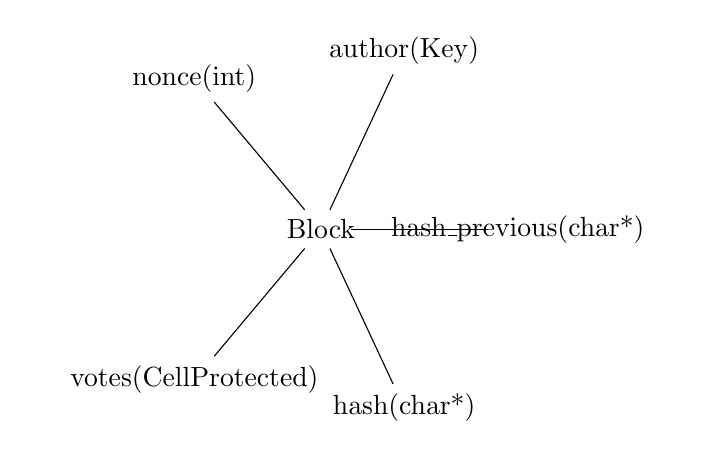
\begin{tikzpicture}[grow cyclic, text width=4cm, align=flush center,
	level 1/.style={level distance=2.5cm,sibling angle=65},
	level 2/.style={level distance=3cm,sibling angle=15}]
\node{Block}
child { node {votes(CellProtected)}}
child { node {hash(char*)}}
child { node {hash\_previous(char*)}}
child { node {author(Key)}}
child { node {nonce(int)}};
\end{tikzpicture}
\begin{lstlisting}[language={C}]
typedef struct block {
    Key *author;
    CellProtected *votes;
    unsigned char *hash;
    unsigned char *previous_hash;
    int nonce;
} Block;
\end{lstlisting}
un bloc contiendra :\newline
— La clé publique de son créateur.\newline
— Une liste de déclarations de vote.\newline
— La valeur hachée du bloc.\newline
— La valeur hachée du bloc précédent.\newline
— Une preuve de travail.\newline
\subsection{la création, l'écriture et la lecture de blocs}
Tout d'abord, nous créons, lisons et écrivons des blocs.
\begin{lstlisting}[language={C}]
void     write_block(char *fileName, Block *block);
Block   *read_block(char *fileName);
void delete_block(Block *b);
void delete_block_partial(Block *b);
Block *create_random_block(Key *author);
Block *init_block(Key *author, CellProtected *lcp);
\end{lstlisting}
\begin{itemize}
\item La fonction create\_random\_block génère un random bloc.
\item La fonction ini\_block initialise un bloc avec nonce=0, l'auteur et les notes comme valeurs d'entrée, toutes les autres sont nulles.
\item La fonction delete\_block supprime un bloc.
\item La fonction delete\_block supprime le bloc ne supprime pas la liste des déclarations
\item La fonction write\_block permet d'écrire dans un fichier un bloc.
\item La fonction read\_block lire un bloc depuis un fichier.
\end{itemize}
Pour tester la validité, nous créons d'abord un bloc aléatoire, puis nous écrivons et lisons les données d'écriture pour créer un nouveau bloc, et enfin nous testons la cohérence des deux blocs.
\subsection{la preuve de travail}
Un système de validation par preuve de travail permettant de repousser, sur un environnement client-serveur.\newline
Pour cela le serveur requiert du client d'effectuer une petite tâche sous forme d'un calcul par exemple. \newline
Bien que cela ne soit pas très grave pour le client, il est impossible de réaliser cette tâche en aussi grand nombre que l'attaque du serveur, car elle serait trop coûteuse en temps et en efforts pour l'attaquant.
\begin{lstlisting}[language={C}]
unsigned char *str_to_SHA256(const char *str);
char *block_to_str(Block *block);
void compute_proof_of_work(Block *B, int d);
int verify_block(Block *, int d);
\end{lstlisting}
\begin{itemize}
\item La fonction block\_to\_str génère une chaîne de caractères
représentant un bloc.
\item La fonction compute\_proof\_of\_work  rendre un bloc valide.
\item La fonction verify\_block vérifie qu’un bloc est valide.
\end{itemize}
Nous convertissons d'abord le bloc en une chaîne de caractères, puis nous générons un hachage à partir de cette chaîne.\newline
Alors on procède par force brute : on commence avec la propriété nonce égale à zéro, puis on augmente le nonce jusqu'à ce que la valeur de hachage du bloc commence par d zéros consécutifs.\newline
La façon dont un bloc prouve sa validité est de savoir si son hachage commence avec d zéros.
\addcontentsline{toc}{paragraph}{Q7.8}
\paragraph*{Q7.8}
Pour tester la fonction computes\_proof\_of\_work et obtenir la meilleure valeur de d, nous générons aléatoirement un bloc et traçons d en fonction du temps de calcul\newline
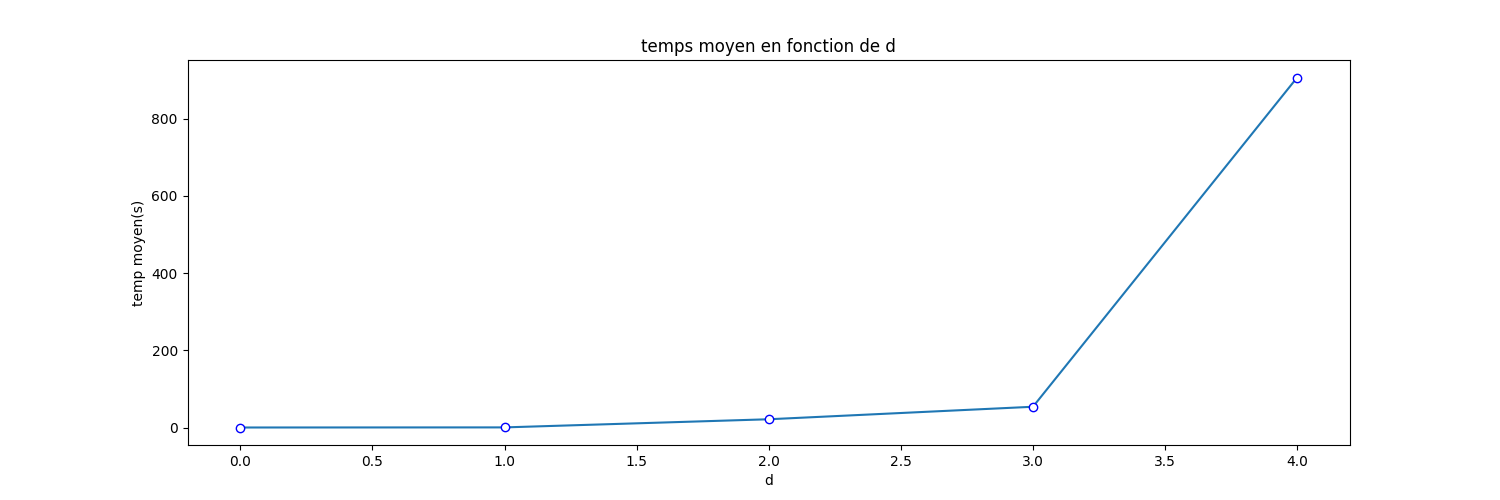
\includegraphics[scale=0.3]{q7_8.png}\newline
Le diagramme montre que pour que le bloc soit infaillible, il faut que d soit supérieur à 4, mais dans nos tests nous avons choisi d=3 afin de réduire le temps d'exécution.
\subsection{Structure arborescente}
Dans une blockchain, chaque bloc contient la valeur hachée du bloc qui le précède,en cas de triche, on peut se retrouver avec plusieurs blocs indiquant le même bloc précédent.Dans cette section on fait confiance à la chaîne la plus longue (en partant de la racine de l’arbre), ce qui permet de retomber sur une chaîne de blocs.
\subsubsection{Manipulation d'un arbre de blocs}
\begin{lstlisting}[language={C}]
typedef struct block_tree_cell {
    Block *block;
    struct block_tree_cell *father;
    struct block_tree_cell *firstChild;
    struct block_tree_cell *nextBro;
    int height;
} CellTree;
CellTree *create_node(Block *b);
int update_height(CellTree *father, CellTree *child);
void add_child(CellTree *father, CellTree *child);
void print_node(CellTree *node);
void print_tree(CellTree *ct);
void delete_node(CellTree *node);
void delete_tree(CellTree *node);
void delete_tree_partial(CellTree *ct);
CellTree *highest_child(CellTree *cell);
CellTree *last_node(CellTree *tree);
CellProtected *fusion(CellProtected *lcp1, CellProtected *lcp2);
CellProtected *longestList(CellTree *tree);
\end{lstlisting}
- La fonction longestList cree de la plus longue chaîne d'un arbre.\newline\newline
Pour tester la validité, nous créons d'abord 10 blocs aléatoires, puis nous formons un arbre avec ces blocs et l'imprimons, nous testons l'arbre pour voir s'il correspond à ce que nous attendions, puis nous testons l'enfant le plus élevé et le dernier nœud, et enfin nous libérons la mémoire.
\addcontentsline{toc}{paragraph}{Q8.8}
\paragraph*{Q8.8}
La fonction fusion(CellProtected *lcp1,CellProtected *lcp2)` mélange deux CellProtected en un seul, dans notre schéma leur complexité est liée à la longueur de la première variable, en supposant que la longueur de `lcp1`' est n, sa complexité est O(n).\newline
Afin de rendre cette fonction O(1), nous pouvons créer une autre structure dans laquelle nous stockons le début et la fin de la liste des chaînes.
\section{ Simulation du processus de vote}
\includegraphics[scale=0.6]{simulation.png}
Dans cette section, nous allons simuler un citoyen qui soumet un vote et un assesseur (citoyen volontaire) qui crée un bloc valide. Nous allons ensuite créer l'arbre de blocs correspondant et calculer le gagnant de l'élection à partir de la plus longue chaîne de l'arbre de confiance.\newline\newline
La chaîne la plus longue de la chaîne de blocs est considérée comme la chaîne valide. En effet, les faux votes sont insérés de manière aléatoire dans un certain sous-arbre, mais il est difficile pour un faussaire de forger directement un plus grand nombre de blocs que le vrai.
\begin{lstlisting}[language={C}]
void submit_vote(Protected *p);
void create_block(CellTree *tree, Key *author, int d);
void add_block(int d, char *name);
CellTree *read_tree();
Key *compute_winner_BT(CellTree *tree, CellKey *candidates, CellKey *voters, int sizeC, int sizeV);
\end{lstlisting}
\begin{itemize}
\item La fonction submit\_vote permettant à un citoyen de soumettre un vote, autrement d’ajouter son vote à la fin du fichier "Pending\_votes.txt".
\item La fonction create\_block :Crée un bloc valide contenant les votes en attente dans le fichier "Pending\_votes.txt", supprime le fichier "Pending\_votes.txt" après avoir créé le bloc, et écrit le bloc obtenu dans un fichier appelé "Pending\_block".

\end{itemize}
Pour vérifier la validité de ces fonctions, nous avons créé une fonction pour simuler l'ensemble du processus électoral et l'avons exécutée dans main.
\begin{lstlisting}[language={C}]
void Simulation(int d,int sizeC,int sizeV);
\end{lstlisting}
La fonction Simulation effectue les étapes suivantes dans l'ordre
\begin{enumerate}
\item générer des données avec 1000 citoyens et 5 candidats (fonction generate\_random\_data).
\item lire les bulletins de vote (fonction read\_protect), les candidats et les citoyens (fonction read\_keys).
\item soumettre tous les votes (fonction submit\_vote) et créer un bloc valide pour chaque 10 votes soumis (fonction create\_block) et ajoutez ensuite le bloc directement au fichier concerné.
\item ajouter la chaîne de blocs (fonction add\_block)
\item lecture (fonction read\_tree) et affichage (fonction print\_tree)
\item calculer et afficher le gagnant (fonction compute\_winner\_BT)
\end{enumerate}
\section{Conclusion}
Dans notre conception, nous utilisons le cryptage rsa pour garantir la confidentialité du vote, la technologie blockchain pour parvenir à un système de vote décentralisé afin de garantir la confiance des électeurs, et la preuve de travail pour réduire considérablement la possibilité de fraude.
\addcontentsline{toc}{paragraph}{Q9.7}
\paragraph*{Q9.7}
Les systèmes de vote électronique basés sur la blockchain permettent aux électeurs de voter à distance, ce qui, d'une part, protège l'identité des électeurs et garantit la confidentialité et, d'autre part, empêche les électeurs de recevoir des interférences pendant le processus de vote. La vérification absolue de tous les bulletins de vote entrant sur la plateforme blockchain est possible, ce qui se traduit par un mécanisme de vote et un contrôle des bulletins sécurisés et transparents, ainsi que par une forte protection contre la fraude électorale.\newline
Si la blockchain peut assurer un certain degré de confidentialité des électeurs et de sécurité des élections après le vote, la nature anonyme des systèmes de vote électronique rend l'identification des électeurs problématique. Des pirates informatiques pourraient potentiellement exploiter les identités des électeurs et interférer avec le processus de vote, tandis que la fiabilité et la sécurité de la plateforme de vote sont également remises en question.\newline
Supposons que les données enregistrées soient valides. Après l'enregistrement du bloc, le pirate peut pirater la base de données et modifier les données du bloc ou ajouter un faux bloc. Le faux bloc a le hash du bloc existant comme hash\_précédent afin d'être ajouté à l'arbre des blocs, supposons que le bloc est A. Si le pirate veut créer un bloc plus long, il doit créer plus de blocs que le sous-arbre de plus grande hauteur de ce bloc A.\newline
Comme nous utilisons la preuve de travail pour valider les blocs, il faut beaucoup de temps pour que ces blocs falsifiés prennent effet, à moins que le bloc A choisi ne se trouve à la fin de l'arbre des blocs.\newline
La combinaison de la preuve du travail et de l'option de la chaîne la plus longue est donc efficace pour réduire la fraude et minimiser son impact sur les résultats, mais n'empêche pas complètement la fraude. Il est tout à fait possible pour les pays et les groupes disposant d'une plus grande puissance de calcul d'interférer avec le déroulement des scrutins s'ils le souhaitent. 

\end{document}